\documentclass{article}
\usepackage{stmaryrd}
\usepackage{graphicx}
\usepackage[utf8]{inputenc}
%\renewcommand*\lightning{\ensuremath{\text{\wasyfamily\char18}}}



\begin{document}
TODO:
\begin{enumerate}
\item Beweis Satz 2.1. umstrukturieren
\item Beweis Satz 3.2. ausschreiben
\item Bekannte Ergebnisse notieren
\item Alg für außenplanare aufarbeiten 
\item Alg. für beliebige $C_j$-Bäume
\item Alg. für Halin Graphen
\end{enumerate}


\section{Definition}
Gegeben sei ein Baum $B=(V,E)$ mit $deg(v_i)\leq 3$ für $v_i \in V$.\\
   Der Graph $G=(V_G,E_G)$ sei wie folgt aus dem Baum $B$ entstanden:\\
   Sei $$V'=\{v_k|v_k \in V \wedge deg(v_k)=3\}\subseteq V$$ eine Menge bestehend aus einer Teilmenge der Knoten in dem Baum $B$. Ersetze jedes Element $v_j \in V'$ durch einen $C_3$ (bezeichne diesen Teilgraphen als \underline{$C_{3,j}$}), so dass jeder Knoten im $C_{3,j}$ mit genau einem der Nachbarn von $v_j$ verbunden ist. Die drei Nachbarn vom $C_{3,j}$ werden dann als die \underline{$C_{3,j}$-$Kinder$} bezeichnet. Sind mind. zwei von den $C_{3,j}$-$Kindern$ Blätter, so bezeichne den $C_{3,j}$ und seine Nachbarn als ein \underline{$Baumblatt(BB)$}. Der \underline{Bifurkator} von $x,y,z$ ist ein Knoten der auf dem kürzesten Wegen von $x$ zu $y$ und zu $z$ liegt, und dabei am weitesten von $x$ entfernt ist.
\subsection{Satz}
Hat ein Graph zwei Teilgraphen $G_R$ und $G_L$, welche durch eine Kante verbunden sind. Gibt es in jedem Teilgraphen mind. einen Knoten aus dem Resolving Set, so ist jedes Knotenpaar $x,y$ getrennt mit der Eigenschaft $x \in G_R$ und $y \in G_L$.
\subsubsection{Beweis}
\begin{center}
  \includegraphics[width=190pt]{bew.pdf}
  \end{center}
  Angenommen, es gibt ein nicht getrenntes Knotenpaar $x,y$. Sei $d_1$ der Bifurkator von $y,x,r_L$ und $d_2$ der Bifurkator von $x,y,r_R$. Dann gilt: $$dist(r_L,x) \leq dist(r_L,d_1)+ dist(d_1,x)$$ $$dist(r_R,y) \leq dist(r_R,d_2)+ dist(d_2,y)$$ $$dist(r_L,y) > dist(r_L,d_1)+ dist(d_2,y)$$ $$dist(r_R,x) > dist(r_R,d_2)+ dist(d_1,x)$$
  Außerdem gilt, da $x$ und $y$ nicht getrennt werden:
   $$dist(r_R,y) =dist(r_R,x),\: dist(r_L,x) = dist(r_L,y)$$ Nun kann eingesetzt und umgeformt werden zu folgendem Widerspruch:
  $$\Rightarrow dist(r_L,d_1)+ dist(d_1,x) \geq dist(r_L,x) = dist(r_L,y)> dist(r_L,d_1)+ dist(d_2,y)$$
  $$\Leftrightarrow dist(r_L,d_1)+ dist(d_1,x) > dist(r_L,d_1)+ dist(d_2,y)$$
  $$\Leftrightarrow dist(d_1,x) >  dist(d_2,y)$$
  
  $$\Rightarrow dist(r_R,y) \leq dist(r_R,d_2)+ dist(d_2,y) < dist(r_R,d_2) + dist(d_1,x) < dist(r_R,x)$$
  $$\Leftrightarrow dist(r_R,y) < dist(r_R,x) = dist(r_R,y)$$
  $$\Leftrightarrow dist(r_R,y) < dist(r_R,y) \lightning $$  
  
\subsection{Satz}
Die Kontraktion von Separationsknoten mit Grad zwei oder das Erweitern mit Separationsknoten mit Knotengrad zwei hat keinen Einfluss auf die Metrische Dimension eines Graphen.
\subsubsection{Beweis}
Gegeben seien ein Separationsknoten $v_s$ mit $deg(v_s)=2$, ein Resolving Set $R_k$ und der Graph $G$ mit Metrischer Dimension $k$. Durch die Separation entstehenden Graphen bezeichne man als $G_R$ und $G_L$. Der Graph $G'$ entsteht durch die Knotenkontraktion von $v_s$ mit einem anderen Knoten. Angenommen es gibt ein Knotenpaar $x,y$, welche im Graphen $G$ unterschiedliche Markierungen hat, und im $G'$ nicht. In $G$ gibt es mind. einen Knoten im $R_K$, der $x,y$ trennt. Sei dies der Knoten $r_k$.\\
\textbf{Fall 1:} Liege $r_k$ im gleichen Teilgraphen wie $x,y$: Der Knoten $v_s$ kann auf keinem kürzesten Weg gewesen sein. So hat seine Kontraktion keinen Einfluss auf die Markierungen und damit ist $R_K$ ein Resolving Set in $G$ genau dann wenn es auch ein Resolving Set in $G'$ ist.\\
\textbf{Fall 2:} Sind $x,y$ in einem anderen Teilgraphen als $r_k$, so liegt $v_s$ auf beiden kürzesten Wegen und so verringern sich beide Markierungen um genau eins. Damit bleiben sie getrennt oder $R_K$ in $G$ ist kein Resolving Set.\\
Sei einer der ursprünglich getrennten Knoten und $r_k$ in dem gleichen Teilgraphen. Sei dies o.B.d.A. der Knoten $x$.\\
\textbf{Fall 3(a):} $G_R$ und $G_L$ sind Wege. Dann gibt es genau einen Knoten im Resolving Set und die Knoten sind getrennt sofern sie zuvor getrennt waren, denn die Metrische Dimension eines Weges ist immer eins.\\
\textbf{Fall 3(b):} O.B.d.A. sei $G_R$ der Teilgraph, der ein Weg ist. Damit besteht das Resolving Set $R_K$ aus mind. 2 Knoten. Ist einer davon im $G_R$, dann gilt das gleiche Argument wie im Fall 3(a) und das Knotenpaar $x,y$ ist getrennt.\\Sind alle Knoten aus dem Resolving Set im $G_L$ und ist die Entfernung von allen Knoten zu $x$ und $y$ gleich im $G'$, so war die Entfernung zu $x$ und zu dem Vorgänger von $y$ gleich, und damit wäre $R_k$ ursprünglich kein gültiges Resolving Set in $G$ gewesen.\\
\textbf{Fall 3(c):} $G_R$ und $G_L$ sind keine Wege. Damit ist in jedem Teilgraphen mind. ein Element aus dem Resolving Set. Der Widerspruch folgt nach Satz 1.1.\\
Für einen eingefügten Knoten geht der Beweis analog.
%\textbf{Angenommen $MD(G')<MD(G)$:}\newline\newline Dann gibt es mind. einen überflüssigen Knoten im $R_K$ mit der Bezeichnung $r_{k'}$. . Seien diese aus dem Resolving Set $R'_K$ entfernt worden. Seien $x,y$ zwei Knoten die im $G$ bzgl. $R'_K$ gleiche Markierungen hatten, und im $G'$ nicht.\\
%Liege $r_{k'}$ im gleichen Teilgraphen wie $x,y$, so kann der Knoten $v_s$ auf keinem kürzesten Weg gewesen sein und so wäre $R_K$ in $G$ ein Resolving Set gewesen.\\
%Sind $x,y$ in einem anderen Teilgraphen als $r_{k'}$, so liegt $v_s$ auf beiden kürzesten Wegen und so verringern sich beide Markierungen um genau eins. Damit bleiben sie getrennt oder $R_K$ in $G$ ist ein Resolving Set.\\
%Sei nun einer der ursprünglich nichtgetrennten Knoten und der trennende Knoten $r_{k+1}$ in dem gleichen Teilgraphen. Sei dies o.B.d.A. $x$.\\
%\textbf{Fall (i):} $G_R$ und $G_L$ sind Wege. Dann gibt es genau einen Knoten im Resolving Set und die Knoten sind getrennt sofern sie zuvor getrennt waren, da die Anzahl der Knoten auf einem Weg irrelevant ist.\\
%\textbf{Fall (ii):} O.B.d.A. sei $G_R$ der Teilgraph, der ein Weg ist. Damit besteht das Resolving Set $r$ aus mind. 2 Knoten. Ist einer davon im $G_R$, dann gilt gleiches Argument wie in Fall (i) und das Knotenpaar $x,y$ ist getrennt.\\Sind alle Knoten aus dem Resolving Set im $G_L$ und ist die Entfernung von allen Knoten zu $x$ und $y$ gleich im $G'$, so war die Entfernung zu $x$ und zu dem Vorgänger von $y$ gleich, und damit wäre $R_k$ ursprünglich kein gültiges Resolving Set.\\
%\textbf{Fall (iii):} $G_R$ und $G_L$ sind keine Wege. Damit ist in jedem Teilgraphen mind. ein Element aus dem Resolving Set. Und die Widerspruch folgt aus nach Satz 1.1.\newline\newline

\section{Separationsknoten mit Grad Zwei}
Bei der Betrachtung, sowie bei der Berechnung der Metrischen Dimension, werden Wege (Knoten mit $deg(v)=2$) miteinander kontrahiert solange bis sie mit einem Knoten mit $deg(v)=3$ oder $deg(v)=1$ kontrahiert wurden. Damit müssen weniger für die Metrische Dimension äquivalente Fälle betrachtet werden, da Knoten mit $deg(v)=2$ nach Satz 1.2 keinen Einfluß auf die Metrische Dimension eines Graphens haben.

\subsection{Beispiele für die Kontraktion}

Beispiel für eine Kontraktion zwischen zwei Baumblättern
\begin{center}
  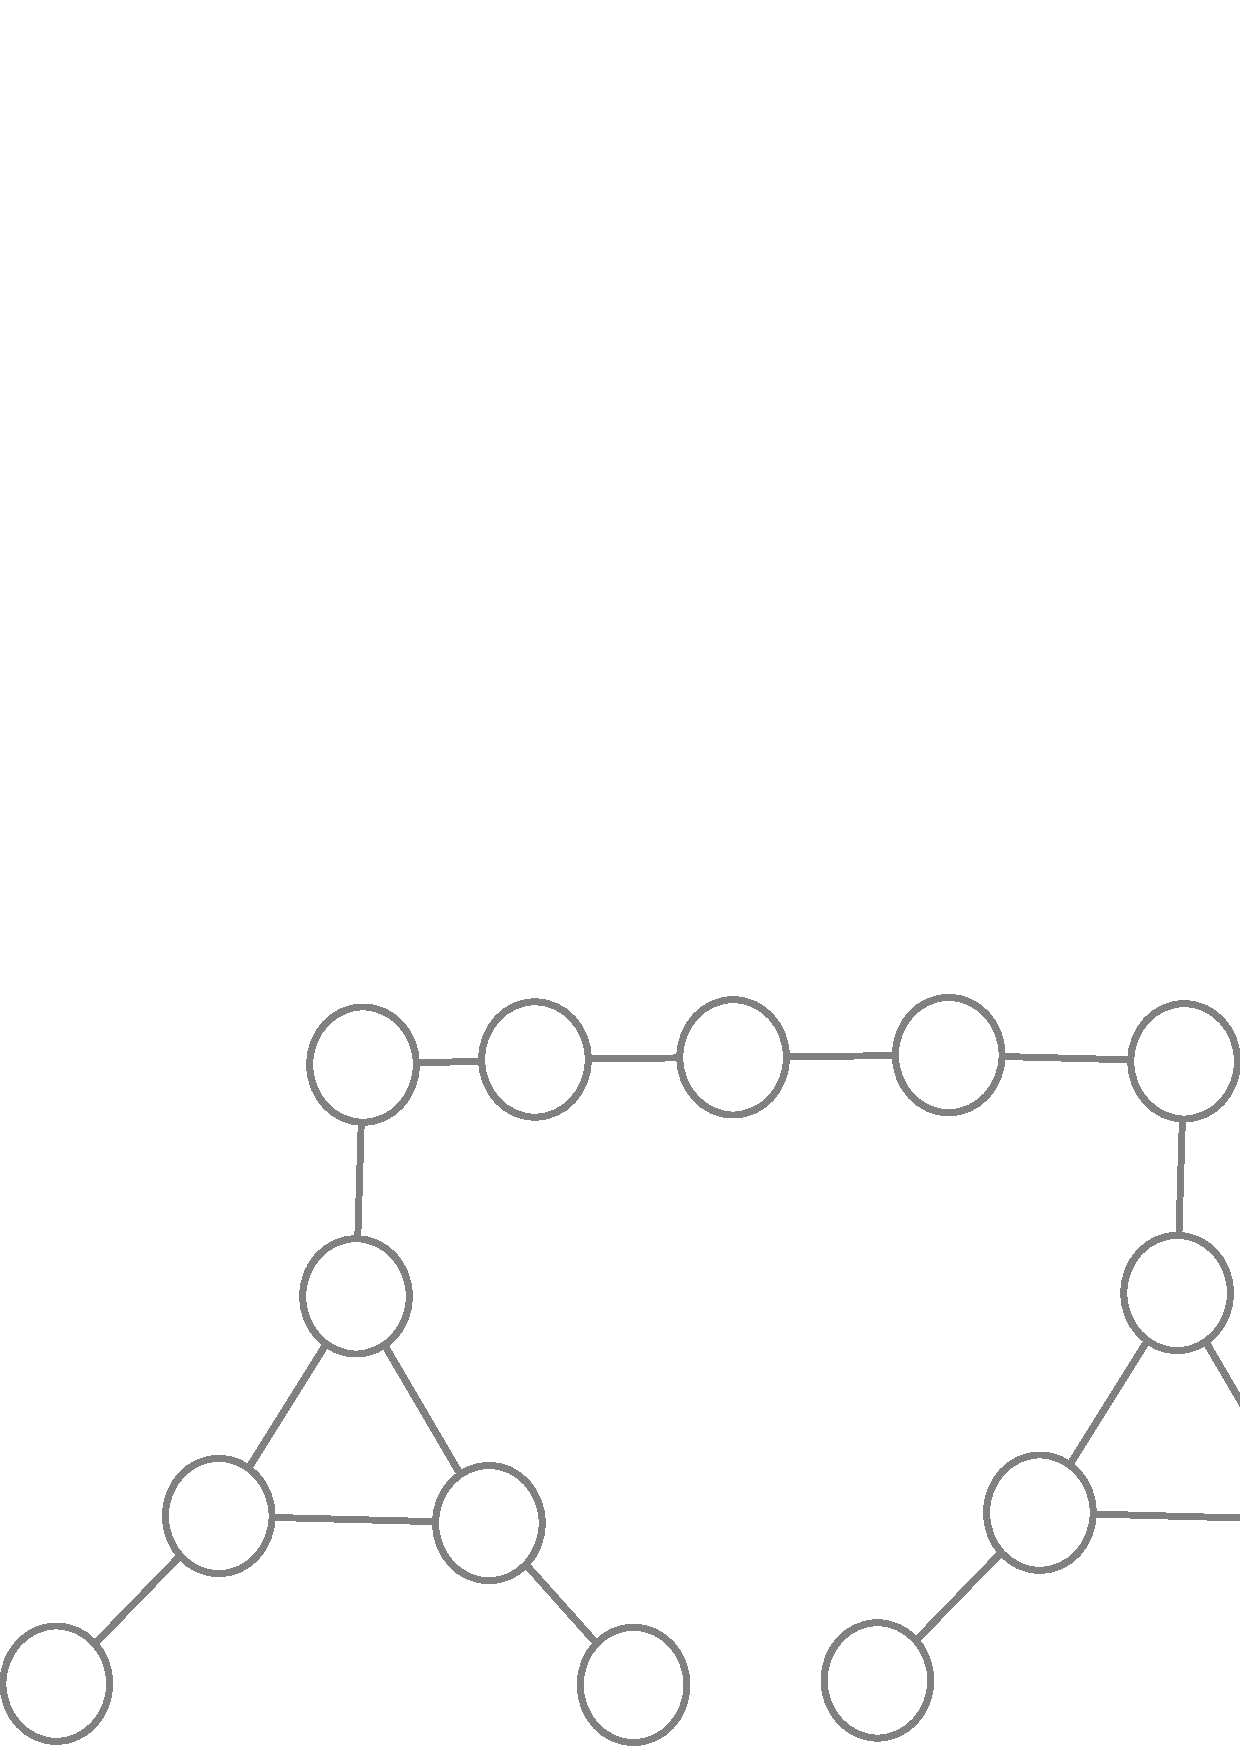
\includegraphics[width=190pt]{impl2.pdf}
  \end{center}
  
Beispiel für eine Kontraktion zwischen einem $C_3$ und einem Blatt
\begin{center}
  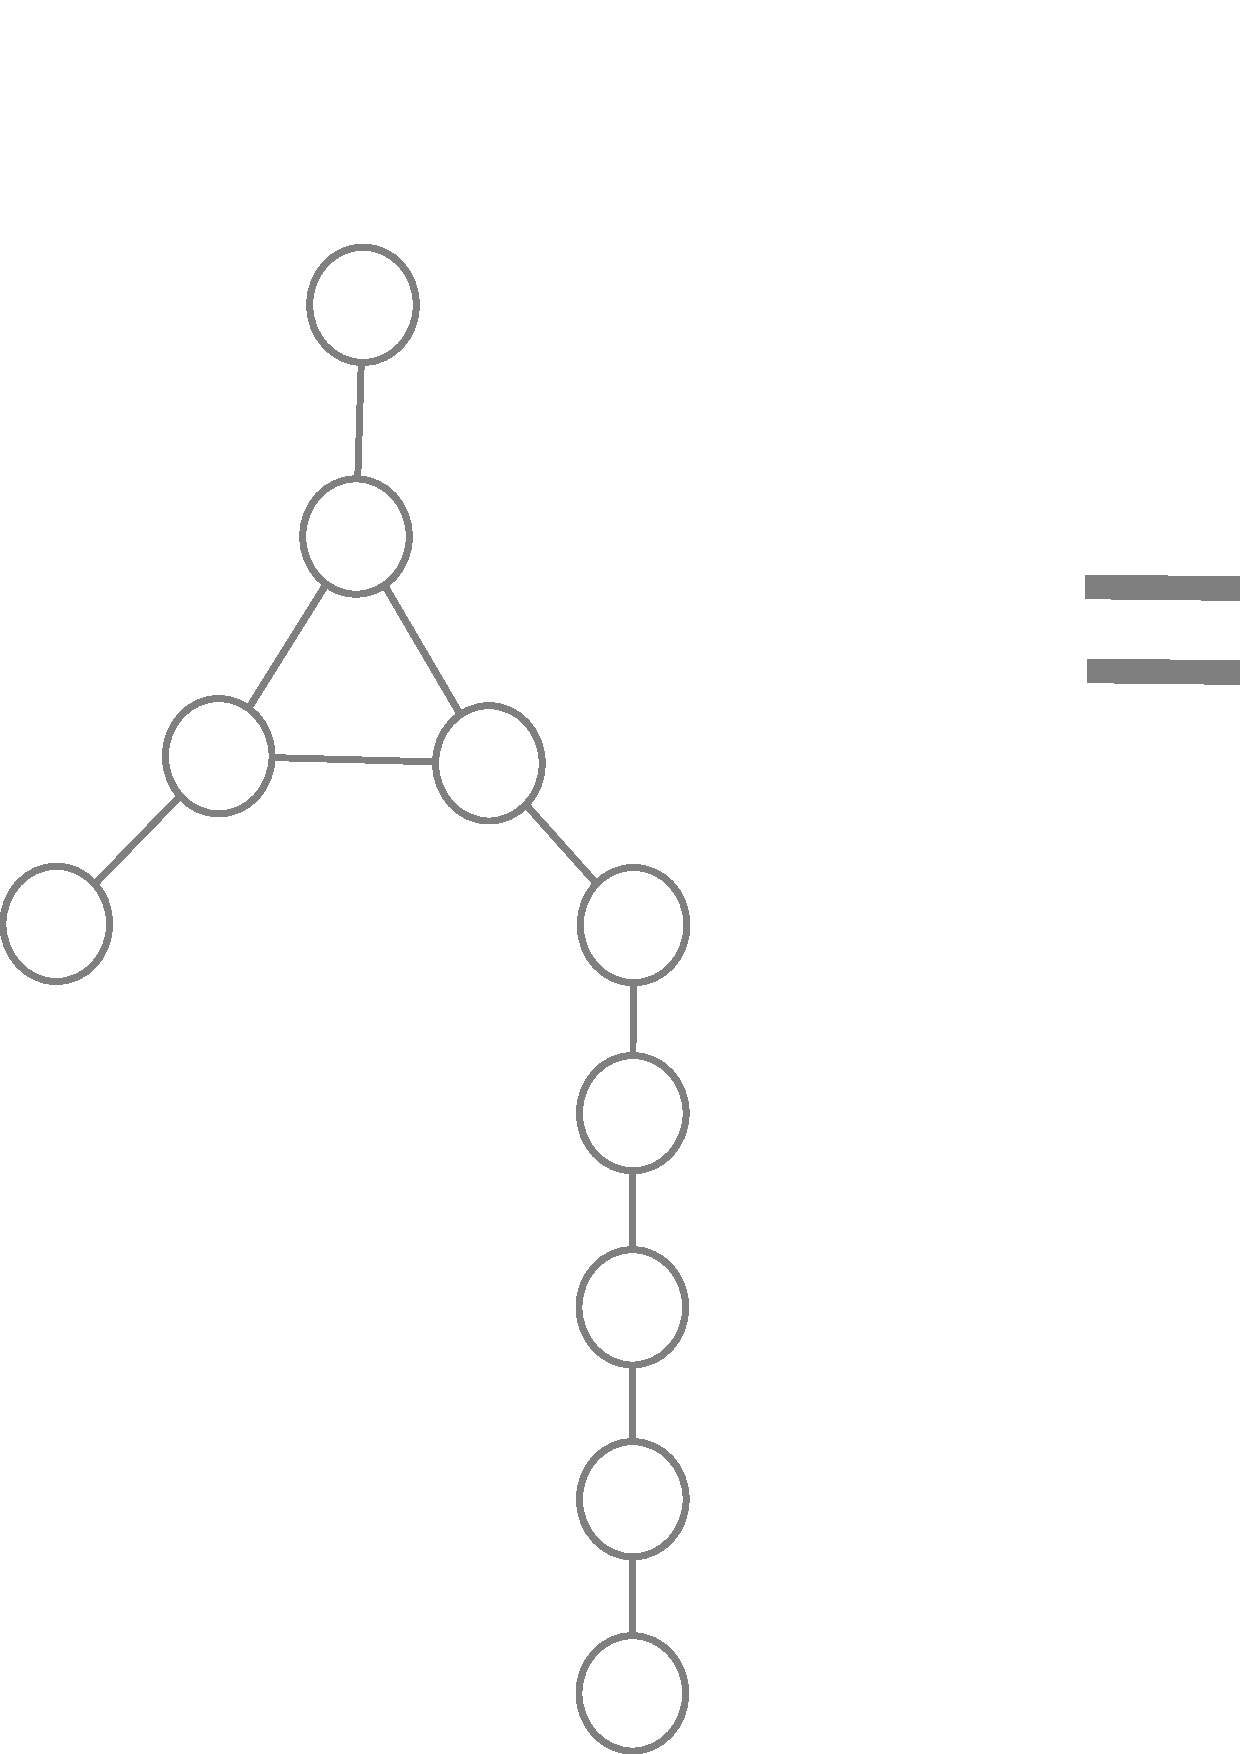
\includegraphics[width=130pt]{impl.pdf}
  \end{center}

\section{Hauptaussage}
Die Metrische Dimension(MD) eines Graphen $G$ mit mindestens zwei $C_{3,j}$ ist gleich der Anzahl seiner Baumblätter.
\subsection{Satz}
Sei $C_{3,j}$ ein beliebiges Baumblatt. In jedem Resolving Set muss mind. einer der Knoten $\{v_{j,1},v_{j,2},v_{j,3},v_{j,4}\}$ enthalten sein.
\subsubsection{Beweis}
Angenommen keiner dieser Knoten ist im Resolving Set. Da die einzige Verbindung zu dem Restgraphen über einen Knoten geht, folgt aus Symmetriegründen, dass die Knoten $v_{j,3}$ und $v_{j,4}$, sowie $v_{j,1}$ und $v_{j,2}$ identische Markierungen haben. Dies widerspricht der Definition eines Resolving Sets.
\begin{center}
\includegraphics[width=170pt]{mm.pdf}
\end{center}
Damit ist die Metrische Dimension(MD) eines Graphen $G$ mit mindestens zwei $C_{3,j}$ mindestens die Anzahl seiner Baumblätter.

\subsection{Satz}
Die Metrische Dimension(MD) eines Graphen $G$ mit mindestens zwei $C_{3,j}$ ist höchstens die Anzahl seiner Baumblätter. Es wird immer das linke Blatt aus jedem Baumblatt in das Resolving Set aufgenommen.
%\subsection{Algorithmus I}
%1. Bestimme alle Baumblätter\\
%2. Nimm genau eines der Blätter eines Baumblattes in das Resolving Set auf.

\subsubsection{Beweis}
Angenommen für einen gebenen Graphen $G$ und sein Resolving Set aus Satz 3.2, gibt es ein nicht getrenntes Knotenpaar $x,y$. 
%IA: Sei $G_2$ ein oben definierter Graph mit genau $|BB|=2$.
%\begin{center}
%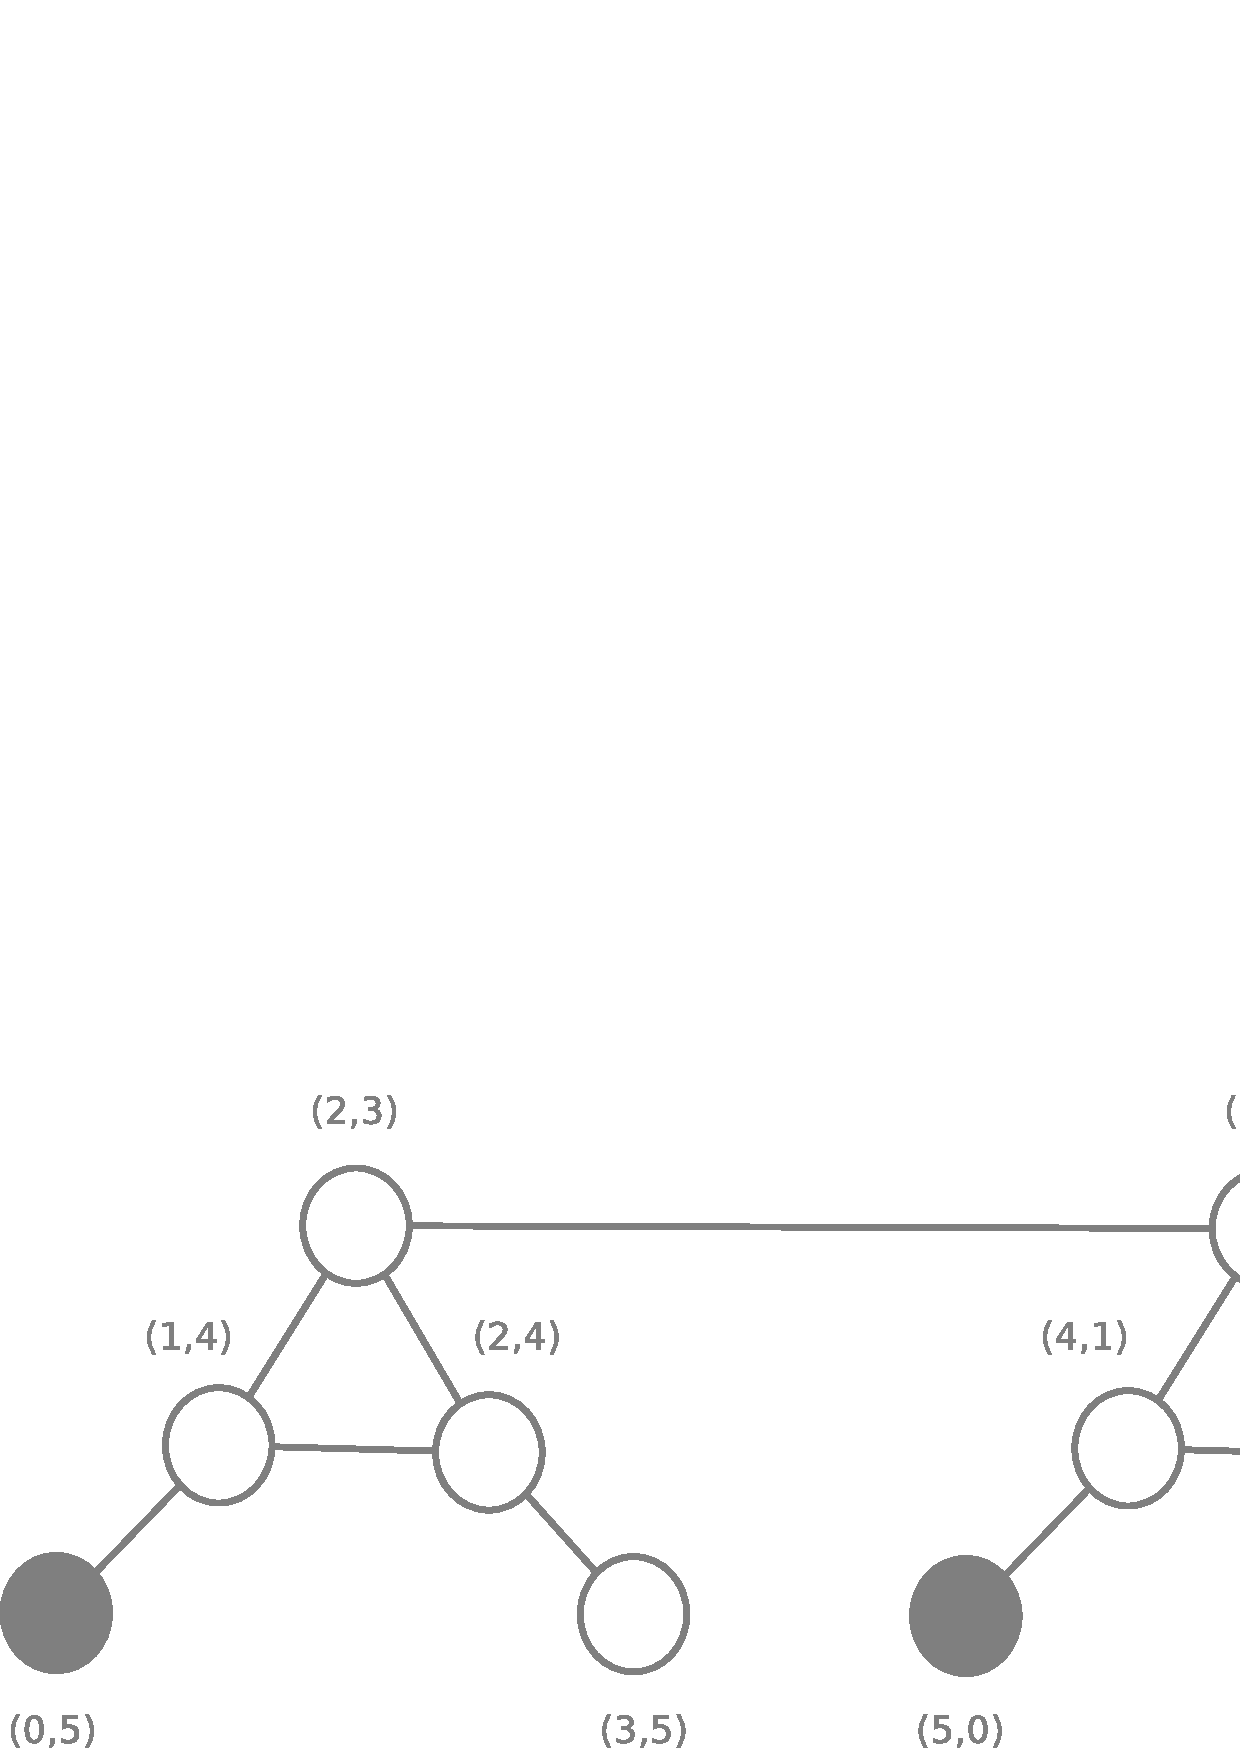
\includegraphics[width=170pt]{G2.pdf}
%\end{center}
%$\Rightarrow MD=2$\newline
%\newline
%IV: $|BB|= MD$\newline
%newline
%IS: ($n\mapsto n+1$) Sei $G_n$ mit $|BB|= n$ gegeben. Betrachte alle Graphen $G_{n+1}$ mit $|BB|=n+1$ und der Graph $G_n$ ist ein Teilgraph.\\
%Es werden zwei Fälle unterschieden:\\
%\textbf{Fall I:} Beim zusätzlichen Baumblatt wird ein Blatt mit einer Kante mit einem Blatt (Knoten $v$ mit $deg(v)=1$) im Graphen $G_n$ verbunden. Alle Knoten $v$ mit $deg(v)=2$ werden entfernt, damit ist das neue Baumblatt Kind eines $C_3$. Dabei darf dieses $C_3$ mit seinen Nachbarn kein Baumblatt in $G_n$ sein, denn sonst wäre die Anzahl der Baumblätter im $G_{n+1}$ immer noch $n$. Die Markierung $(a)=\{a_1, a_2, \ldots, a_n\}$ ist die Länge der kürzesten Wege zu den Knoten im Resolving Set $r_n$ im Graphen $G_n$ bestehend aus $n$ Komponenten. Dabei ist sein Nachfolger $(a+1)=\{a_1+1, a_2+1, \ldots, a_n+1\}$. Im Graphen $G_{n+1}$ gibt es zwei Knotenpaare die von dem Resolving Set $r_n$ nicht getrennt werden. Durch die Aufnahme eines Knotens (der graumarkierte Knoten in der Abbildung) ist die neue Menge $r_{n+1}$ ein Resolving Set des Graphens $G_{n+1}$. 
%\begin{center}
%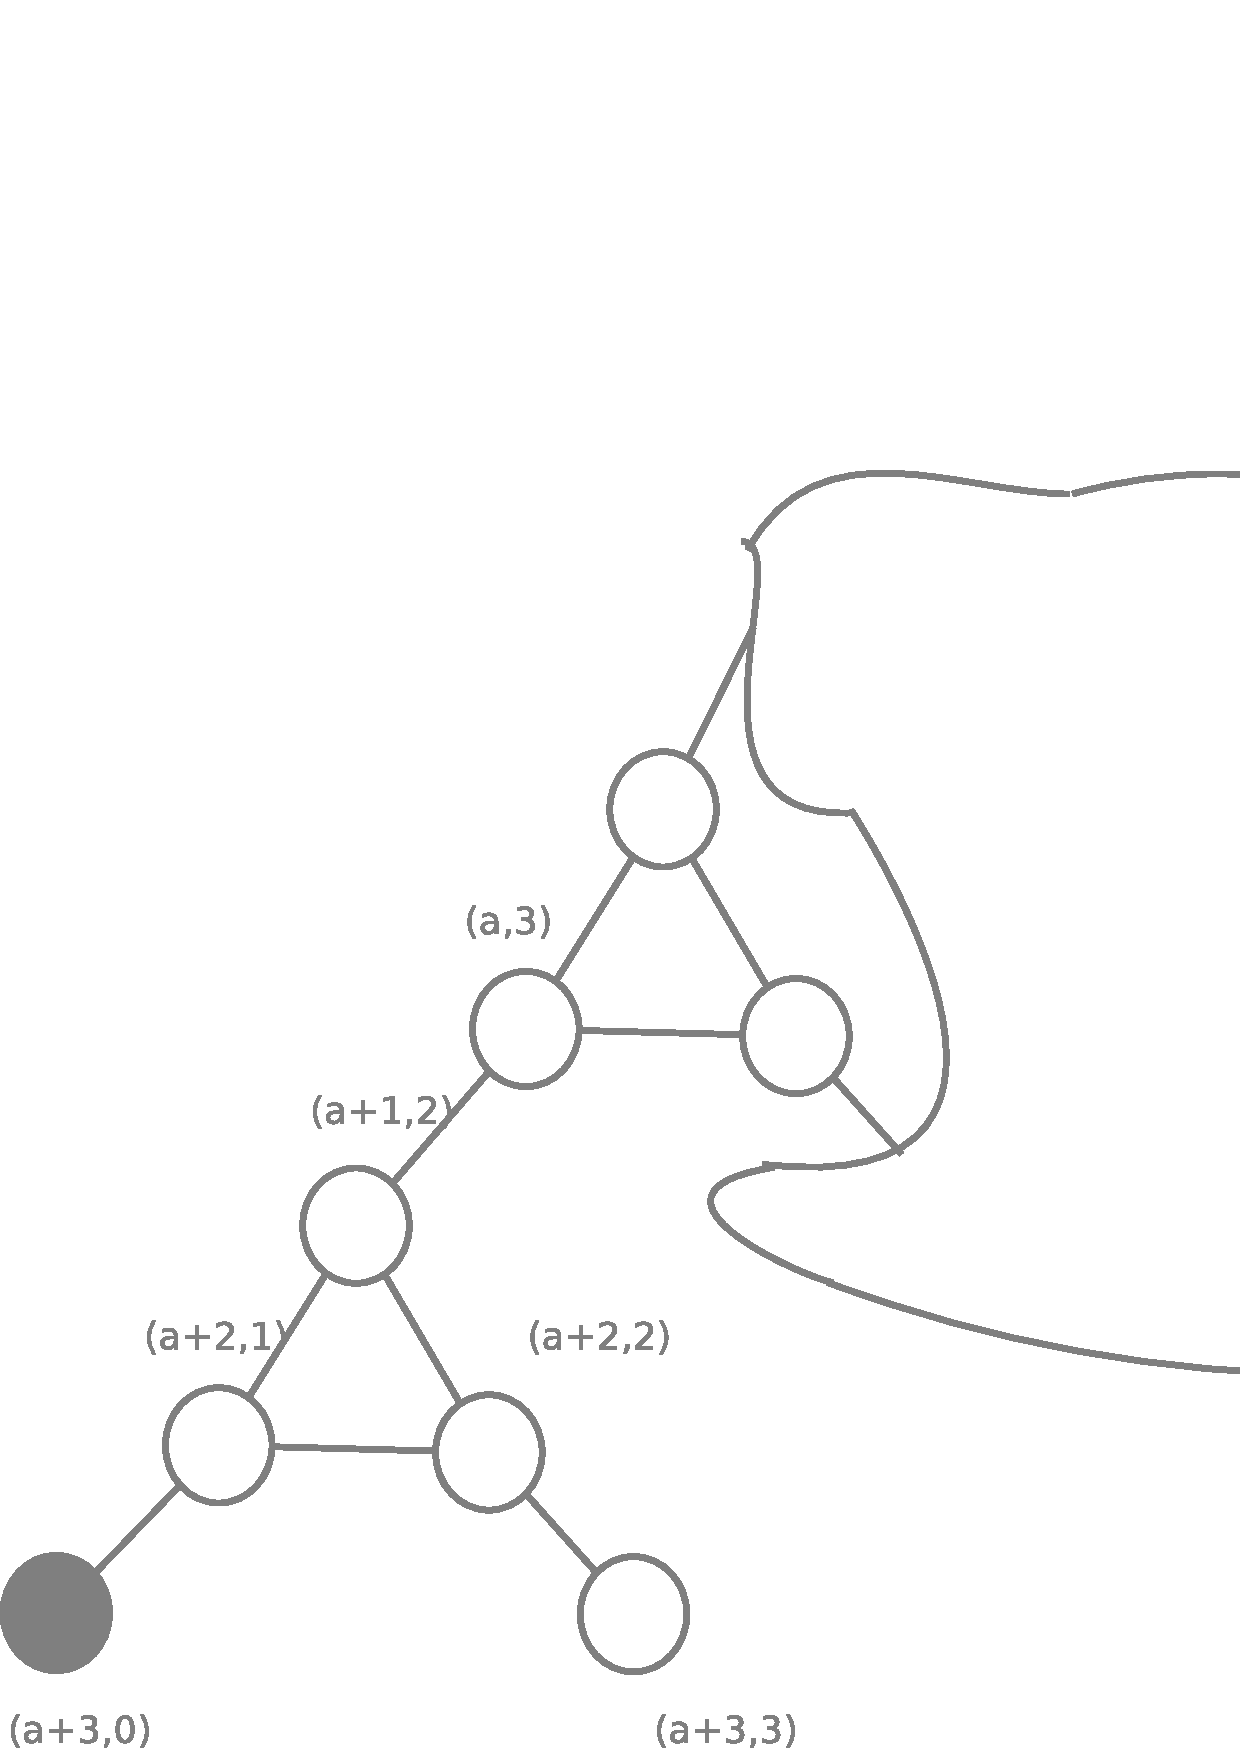
\includegraphics[width=170pt]{fall1.pdf}
%\end{center}
%$\Rightarrow MD(G_{n+1})=MD(G_n)+1=n+1$\newpage
%\textbf{Fall II:} Das Baumblatt kommt an einen Knoten mit Grad 2. Dabei müssen auf beiden Seiten in den Teilgraphen es mind. ein Baumblatt geben, sonst tritt Fall 1 ein, oder die Anzahl der Baumblätter im $G_{n+1}$ bleibt $n$.
%\begin{center}
%\includegraphics[width=260pt]{lala.pdf}
%\end{center}
%$\Rightarrow MD(G_{n+1})=MD(G_n)+1=n+1$\newline
%\newline
%Das Baumblatt kann zu keinem Knoten mit Grad 3 verbunden werden, denn sonst hätte der resultierende Knoten Grad 4.
\section{Sonderfälle}
Fall I: Der Baum besteht nur aus Knoten mit $deg(v) \leq 2$. Damit ist er ein Weg und seine Metrische Dimension ist eins.\\
Fall II: Der Baum beinhaltet genau einen Knoten mit $deg(v)=3$. Seine Metrische Dimension ist zwei.


\end{document}
